\subsubsection{Impact of Different Types of Program Graphs}
\label{sec:graphs}

\begin{figure}[thbp]
\begin{center}
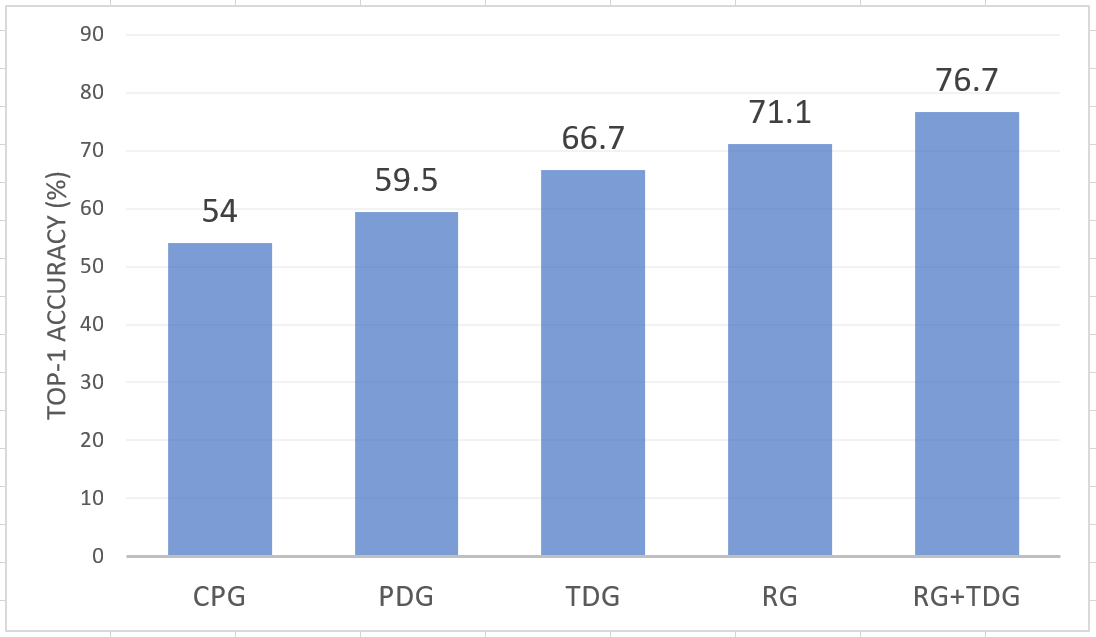
\includegraphics[width=2.8in]{figures/sensi-graphs-name}
\vspace{-8pt}
\caption{RQ3. Impact of Input Graph on Variable Name Prediction}
\label{graph-name-result}
{\bf CPG}: Code Property Graph, {\bf PDG}:Program Dependence Graph, {\bf TDG}: Type Dependency Graph, {\bf RG}:Relation Graph. 
\end{center}
\end{figure}

\begin{figure}[thbp]
\begin{center}
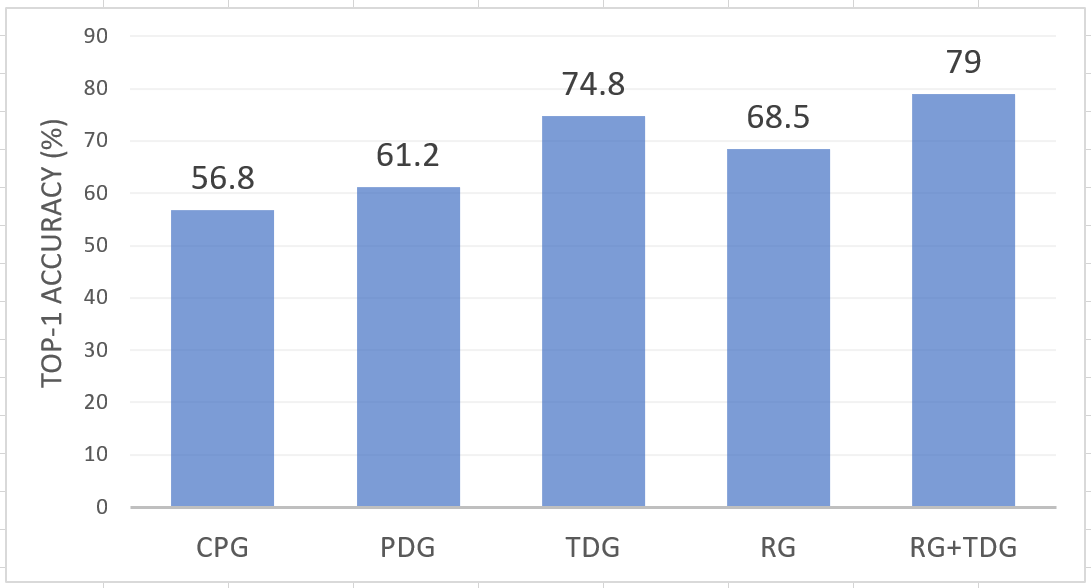
\includegraphics[width=2.8in]{figures/sensi-graphs-type}
\vspace{-8pt}
\caption{RQ3. Impact of Input Graph on Variable Type Prediction}
\label{graph-type-result}
{\bf CPG}: Code Property Graph, {\bf PDG}:Program Dependence Graph, {\bf TDG}: Type Dependency Graph, {\bf RG}:Relation Graph.
\end{center}
\end{figure}

As in any approach, the representation for source code is important
and affects the final performance. In this experiment, we kept the
same neural network architecture, however, changed different input
graphs extracted from source code. In addition to the graphs used in
{\tool} (relation graph (RG), type dependency graph (TDG)), we also
experimented with program dependence graph (PDG) and code property
graph (CPG)~\cite{CPG-2014} because they are popularly used in several
machine learning approaches for source code.

As seen in Figure~\ref{graph-name-result} and
Figure~\ref{graph-type-result}, for variable name prediction, RG helps
the model more than TDG and for variable type prediction, TDG helps
the model more than RG. This is expected because each of them is
designed toward capturing the key features for its problem. For the
dual tasks, the combined graph (RG+TDG) in {\tool} yields the highest
accuracies in both name prediction and type prediction. In contrast,
PDG capturing the dependencies among statements/expressions are not
specifically designed for handling variable names/types, thus, did not
yield high accuracy as TDG, RG, and CG. An interesting observation is
that CPG, which contains lexical, syntax, and dependency information,
did not help the model as much as PDG and others. It seems that CPG
contains too much irrelevant information for name/type prediction.



%1. Code property graph is complex but cannot represent the variable relationships and type changes clearly (EEGCN+GCNmf+CPG compared with EEGCN+GCNmf+RG on name prediction; EEGCN+GCNmf+CPG compared with EEGCN+GCNmf+TDG on type prediction)


